\documentclass[12pt,openany, tikz,border=10pt]{book}


% Load packages
\usepackage[utf8]{inputenc} % for unicode input
\usepackage{geometry} % for page layout
\usepackage{hyperref} % for hyperlinks
\usepackage{tocbibind} % includes the bibliography in the table of contents
\usepackage{amsmath} % for advanced math formatting
\usepackage{amsfonts} % for mathematical fonts
\usepackage{amssymb} % for mathematical symbols
\usepackage{lipsum} % generates filler text
\usepackage{fancyhdr}
\usepackage{amsthm} % for theorem environments
\usepackage{amsmath}
\usepackage[table]{xcolor} % for cell coloring
\usepackage{colortbl} % for cell coloring
\usepackage{graphicx} % for scaling the table
\usepackage{booktabs} % For professional looking tables
\usepackage[table]{xcolor} % For cell coloring
\usepackage[normalem]{ulem} % For underlining
\usepackage[document]{ragged2e}
\usepackage{tikz}
\usepackage{algorithm}
\usepackage{algpseudocode}
\usepackage{wrapfig}

\usetikzlibrary{arrows.meta,calc,decorations.markings,math,arrows.meta}

% Document geometry (page size, margins)
\geometry{a4paper, left=25mm, right=25mm, top=30mm, bottom=30mm}
% Custom page style for centered page numbers
\pagestyle{fancy}
\fancyhf{} % clear all header and footer fields
\fancyfoot[C]{\thepage} % center page number
\renewcommand{\headrulewidth}{0pt}
\renewcommand{\footrulewidth}{0pt}



% Document begins
\begin{document}


% Title Page
\begin{titlepage}
    \centering
    \vspace*{1cm}
    
    
    \vspace{0.5cm}
    \Huge
    Fundamentals of digital systems
    \vspace{10px}
    \newline
    \text{ \large Ali EL AZDI}


    \text{ \Large IC BA2 - Mirjana Stojilović}
    
    \vfill
    \large
    February 19, 2024

    
\end{titlepage}
\begin{center}
    \vspace*{1cm}
    \textbf{Introduction}
    \newline
    \paragraph[short]{}{This document is designed to offer a LaTeX-styled overview of the Fundamentals of Digital Systems course, emphasizing brevity and clarity. Should there be any inaccuracies or areas for improvement, please do not hesitate to reach out to me at ali.elazdi@epfl.ch for corrections. Hoping to provide an experience similar to the one provided by past generations of students in other subjects. }
\end{center}


% Table of Contents
\tableofcontents

% List of Figures (Uncomment if needed)
% \listoffigures

% List of Tables (Uncomment if needed)
% \listoftables

\mainmatter% Chapter 1
\chapter{Number Systems}


% Section 1.1
\section{Digital Representations}
\begin{itemize}
    \item[] In a digital representation, a number is represented by an ordered n-tuple:
    \begin{itemize}
        \item[] The n-tuple is called a \textbf{digit vector}, each element is a \textbf{digit}
        \item[] The number of digits $n$ is called the precision of the representation. (careful! leftward indexing)
        
    
    \end{itemize}
\end{itemize}
\[ X  = (X _{n-1}, X _{n-1}, \ldots, X _{0}) \]
\begin{itemize}
    \item[] Each digit is given \textbf{a set of values} $D_{i}$ 
    (eg. For base 10 representation of numbers, $D_i = \{0,1,2, \dots, 9\}$)
    \item[] The \textbf{set size}, the maximum number of representable digit vectors is: $K = \prod_{i=0}^{n-1} |D_{i}|$
\end{itemize}



  
  




\subsection{(Non)Redundant Number Systems}
     A number system is nonredundant if each digit-vector represents a different integer

\subsection{Weighted Number Systems}
The rule of representation if a Weighted (Positional) Number Systems is as follows :
$$\;\displaystyle\sum_{i=0}^{n-1} X_{i}W_{i}$$ where $$W = (W_{n-1}, W_{n-2}, \dots, W_{0})$$

\subsection{Radix Systems}
When weights are in this format : 
\[
\begin{cases}
   $$W_{0} = 1 \\
    W_{i+1} = W_{i}R_{i} \;\; \text{with } 1 \leq i \leq n-1$$
    \end{cases} \]





Also written :
$W_{0} = 1, \; \prod_{j=0}^{i-1} R_{j}$

\subsection{Fixed and Mixed-Radix Number Systems}
\begin{itemize}
    \item[] In a \textbf{fixed-radix system}, all elements of the radix-vector have the same value \( r \) (\textit{the radix})
    \item[] The weight vector in a fixed-radix system is given by:
    \begin{equation*}
      W = \left( r^{n-1}, r^{n-2}, \ldots, r^2, r, 1 \right)
    \end{equation*}
    and the integer \( x \) becomes:
    \begin{equation*}
      x = \sum_{i=0}^{n-1} X_i \times r^i
    \end{equation*}
    \item[] In a \textbf{mixed-radix system}, the elements of the radix-vector differ
  \end{itemize}
  \subsection*{Example: Decimal Number System}
The decimal number system has the following characteristics:
\begin{itemize}
    \item[-] Radix \(r = 10\), it's a fixed-radix system.
\end{itemize}
The weight vector \(W\) is defined as:
\begin{equation*}
    W = \left(10^{n-1}, 10^{n-2}, \ldots, 10^2, 10, 1\right)
\end{equation*}
An integer \(x\) in this system is represented by:
\begin{equation*}
    x = \sum_{i=0}^{n-1} X_i \times 10^i
\end{equation*}
For example:
\begin{equation*}
    854703 = 8 \times 10^5 + 5 \times 10^4 + 4 \times 10^3 + 7 \times 10^2 + 0 \times 10^1 + 3 \times 10^0
\end{equation*}

\subsubsection{Examples of Fixed and Mixed radix systems}
\begin{description}
  \item[Fixed:] The base of number systems.
  \begin{itemize}
      \item Decimal – radix 10
      \item Binary – radix 2
      \item Octal – radix 8
      \item Hexadecimal – radix 16
  \end{itemize}
  \item[Mixed:] An example of a mixed radix representation, such as time:
  \begin{itemize}
      \item Radix-vector \(R = (24, 60, 60)\)
      \item Weight-vector \(W = (3600, 60, 1)\)
  \end{itemize}
\end{description}

\subsection{Canonical Number Systems}

\begin{itemize}
  \item[] In a \textbf{canonical number system}, the set of values for a digit \( D_i \) is with \( |D_i| = R_i \), the corresponding element of the radix vector
  \begin{equation*}
    D_i = \{0, 1, \ldots, R_i - 1\}
  \end{equation*}
  \item[] Canonical digit sets with fixed radix:
  \begin{itemize}
    \item Decimal: \{0, 1, \ldots, 9\}
    \item Binary: \{0, 1\}
    \item Hexadecimal: \{0, 1, 2, \ldots, 15\}
  \end{itemize}
  \item[] Range of values of \( x \) represented with \( n \) fixed-radix-\( r \) digits:
  \begin{equation*}
    0 \leq x \leq r^n - 1
  \end{equation*}
  A system with fixed positive radix r and a canonical set of digit values is called a radix-r conventional number system.
\end{itemize}
\newpage
\section{Binary/Octal/Hexadecimal to/from Decimal}
\section*{Conversion Table}
\begin{itemize}
  \item[] The hexadecimal system supplements 0-9 digits with the letters A-F.
  \vspace{-5px}
  \item[] \textit{Remark.} Programming languages often use the prefix 0x to denote a hexadecimal number.
\end{itemize}

% Define the color for the table cells
\definecolor{cellblue}{rgb}{0.88, 0.94, 0.97}
\definecolor{cellpink}{rgb}{0.96, 0.88, 0.89}
\definecolor{cellgreen}{rgb}{0.906, 1, 0.831}
\vspace{-20px}

\begin{table}[ht]
    \centering
    \caption{Conversion table up to 15.}
    \vspace{10px}
    \label{my-label}
    \begin{tabular}{@{}cccc@{}}
    \toprule
    \textbf{Decimal} & \textbf{Binary} & \textbf{Octal} & \textbf{Hexadecimal} \\ \midrule
     0 & \cellcolor{cellgreen}0000 & \cellcolor{cellblue}00 & \cellcolor{cellpink}0 \\
     1 & \cellcolor{cellgreen}0001 & \cellcolor{cellblue}01 & \cellcolor{cellpink}1 \\
     2 & \cellcolor{cellgreen}0010 & \cellcolor{cellblue}02 & \cellcolor{cellpink}2 \\
     3 & \cellcolor{cellgreen}0011 & \cellcolor{cellblue}03 & \cellcolor{cellpink}3 \\
     4 & \cellcolor{cellgreen}0100 & \cellcolor{cellblue}04 & \cellcolor{cellpink}4 \\
     5 & \cellcolor{cellgreen}0101 & \cellcolor{cellblue}05 & \cellcolor{cellpink}5 \\
     6 & \cellcolor{cellgreen}0110 & \cellcolor{cellblue}06 & \cellcolor{cellpink}6 \\
     7 & \cellcolor{cellgreen}0111 & \cellcolor{cellblue}07 & \cellcolor{cellpink}7 \\
     8 & \cellcolor{cellgreen}1000 & \cellcolor{cellblue}10 & \cellcolor{cellpink}8 \\
     9 & \cellcolor{cellgreen}1001 & \cellcolor{cellblue}11 & \cellcolor{cellpink}9 \\
    10 & \cellcolor{cellgreen}1010 & \cellcolor{cellblue}12 & \cellcolor{cellpink}A \\
    11 & \cellcolor{cellgreen}1011 & \cellcolor{cellblue}13 & \cellcolor{cellpink}B \\
    12 & \cellcolor{cellgreen}1100 & \cellcolor{cellblue}14 & \cellcolor{cellpink}C \\
    13 & \cellcolor{cellgreen}1101 & \cellcolor{cellblue}15 & \cellcolor{cellpink}D \\
    14 & \cellcolor{cellgreen}1110 & \cellcolor{cellblue}16 & \cellcolor{cellpink}E \\
    15 & \cellcolor{cellgreen}1111 & \cellcolor{cellblue}17 & \cellcolor{cellpink}F \\\bottomrule
    \end{tabular}
    \end{table}
    

    \subsection{Convertion examples}    
    \subsubsection*{Binary to Decimal:}

    
      To convert a binary number to decimal, multiply each bit by two raised to the power of its position number, starting from zero on the right.



    \begin{flalign*}
    & \text{Binary:}       & \underline{1} \underline{0} \underline{1} \underline{1} & \\
    & \text{Decimal:}      & 1 \times 2^3 + 0 \times 2^2 + 1 \times 2^1 + 1 \times 2^0 = 8 + 0 + 2 + 1 = 11 &
    \end{flalign*}
    
    \newpage

    \subsubsection*{Decimal to Binary:}

    Let's convert the decimal number \( 25_{10} \) to binary.

    \begin{tabular}{rclr}
    $25 \div 2$ & = & 12 & remainder 1 (LSB) \\
    $12 \div 2$ & = & 6  & remainder 0 \\
    $6 \div 2$  & = & 3  & remainder 0 \\
    $3 \div 2$  & = & 1  & remainder 1 \\
    $1 \div 2$  & = & 0  & remainder 1 (MSB) \\
    \end{tabular}

    \vspace*{10px}
    Thus, the binary representation of \( 25_{10} \) is \( 11001_2 \) (reading the remainders in reverse).
   

    \vspace*{10px}
    \textit{Personal Remark} The trick is always to try to answer the question, what's the biggest power of 2 I need to form the number?. For 157, the biggest power would be $2^{7} = 128$, then $128+64$ is greater than 157, $128 + 32$ is still greater than 157, $128 + 16 = 144$, and so on to obtain : $128+16+8+4+1=157$ which can be written as $2^7 + 2^4 + 2^3 + 2^2 + 2^0 = 157$. Written in binary as $ 10011101_{2} $

    \subsubsection*{Octal to Decimal:}
    
    Each octal digit is converted to decimal by multiplying it by eight raised to the power of its position number, starting from zero on the right.
    
    \begin{flalign*}
    & \text{Octal:}        & \underline{2} \underline{5} \underline{7} & \\
    & \text{Decimal:}      & 2 \times 8^2 + 5 \times 8^1 + 7 \times 8^0 = 128 + 40 + 7 = 175 &
    \end{flalign*}
    \subsubsection*{Decimal to Octal:}
 To convert the decimal number \(93_{10}\) to octal.
    
    \begin{tabular}{rclr}
    $93 \div 8$ & = & 11 & remainder 5 \\
    $11 \div 8$ & = & 1  & remainder 3 \\
    $1 \div 8$  & = & 0  & remainder 1 \\
    \end{tabular}
    
    \vspace*{10px}
    Thus, the octal representation of \(93_{10}\) is \(135_8\) (reading the remainders in reverse).
    
    \subsubsection*{Hexadecimal to Decimal:}

    To convert the hexadecimal number \( \text{1A3}_{16} \) to decimal.

    \begin{flalign*}
    & \text{Hexadecimal:}       & \underline{1} \underline{A} \underline{3} & \\
    & \text{Decimal:}           & 1 \times 16^2 + A \times 16^1 + 3 \times 16^0 & \\
    &                           & 1 \times 256 + 10 \times 16 + 3 \times 1 & \\
    &                           & 256 + 160 + 3 & \\
    &                           & 419 &
    \end{flalign*}

    Here, \( \text{A} \) in hexadecimal corresponds to \( 10 \) in decimal.



    


    
    \subsubsection*{Decimal to Hexadecimal:}
  
    To convert the decimal number \(291_{10}\) to hexadecimal.
    
    \begin{tabular}{rclr}
    $291 \div 16$ & = & 18 & remainder 3 \\
    $18 \div 16$  & = & 1  & remainder 2 \\
    $1 \div 16$   & = & 0  & remainder 1 \\
    \end{tabular}
    
    \vspace*{10px}
    Thus, the hexadecimal representation of \(291_{10}\) is \(123_{16}\) (reading the remainders in reverse).
    


    \section{Octal/Hexadecimal to/from Binary}
    \section*{Bit-Vector Representation Summary}

    \begin{itemize}
      \item Digit-vectors for binary, octal, and hexadecimal systems are represented using bit-vectors. In binary, 0 and 1 are directly represented as 0 and 1.
      \item In systems like octal or hexadecimal, a digit is a bit-vector of length \( k \), where \( k \) is the number of bits needed to represent the base.$$k=\log_{2}(r)$$
      with r the radix of the system (eg. 8 for octal convertion).
      \item For example, the hexadecimal digit \( B \) is represented as the bit-vector 1101 in binary. \textit{We obtain a length 4 bit-vector because the base is 16 and \( \log_{2}(16) = 4 \)}
    \end{itemize}

    \subsubsection*{Binary to Octal:}

    To convert a binary number to octal, group every three binary digits into a single octal digit, because \( k = \log_2 8 = 3 \).
    
    \begin{flalign*}
    & \text{Binary:}       & \underline{010}\,\underline{000}\,\underline{100}\,\underline{110} & \\
    & \text{Octal:}        & 2_8\,0_8\,4_8\,6_8 &
    \end{flalign*}
    
    \subsubsection*{Binary to Hexadecimal:}
    
    To convert a binary number to hexadecimal, group every four binary digits into a single hexadecimal digit, because \( k = \log_2 16 = 4 \).
    
    \begin{flalign*}
    & \text{Binary:}       & \underline{1011}\,\underline{1110}\,\underline{1010}\,\underline{1101} & \\
    & \text{Hexadecimal:}  & B_{16}\,E_{16}\,A_{16}\,D_{16} &
    \end{flalign*}
    


    \subsubsection*{Octal to Hexadecimal:}
    Convert the octal number to binary, then group the binary digits in sets of four and convert each group to its hexadecimal equivalent.
    
    \begin{flalign*}
    & \text{Octal:}        & \underline{2} \underline{5} \underline{7} & \\
    & \text{Binary:}       & 010 \, 101 \, 111 & \text{ (Octal to binary)} \\
    & \text{Binary grouped:} & \underline{0101} \, \underline{0111} & \\
    & \text{Hexadecimal:}  & 5 \, 7 & \text{ (Binary to hexadecimal)}
    \end{flalign*}    

    \section{Representation of
    Signed Integers}
    \subsection{Sign-Magnitude Representation (SM)}

    A signed integer \( x \) is represented by a pair \( (x_s, x_m) \), where \( x_s \) is the \textit{sign} and \( x_m \) is the \textit{magnitude} (positive integer).

    \begin{itemize}
        \item[] The sign (positive, negative) is represented by a the most significant bit (MSB) of the digit vector:
        \begin{itemize}
            \item[] \( 0 \rightarrow \) positive
            \item[] \( 1 \rightarrow \) negative
        \end{itemize}
        \item[] The magnitude can be represented as any positive integer. In a conventional radix-\( r \) system, the range of \( n \)-digit magnitude is:
        \[ 0 \leq x_m \leq r^n - 1 \]
    \end{itemize}

    \begin{itemize}
      \item[-] Examples:
      \begin{align*}
          01010101_2 &= +85_{10} \\
          01111111_2 &= +127_{10} \\
          00000000_2 &= +0_{10} \\
          11010101_2 &= -85_{10} \\
          11111111_2 &= -127_{10} \\
          10000000_2 &= -0_{10} \\
      \end{align*}
  \end{itemize}
  \newpage
  Note: The Sign-and-Magnitude representation is considered a redundant system because both \( 00000000_2 \) and \( 10000000_2 \) represent zero.

  \begin{itemize}
    \item[] \textit{SM} consists of an equal number of positive and negative integers.
    \item[] An \( n \)-bit integer in sign-and-magnitude lies within the range \textit{(because of 0's double representation and that MSB is used for the sign)}: 
    $$ [-\left(2^{n-1} - 1\right), +\left(2^{n-1} - 1\right)] $$ 
    \item[] Main disadvantage of SM: complex digital circuits for arithmetic operations (addition, subtraction, etc.).
\end{itemize}

\section{True-and-Complement (TC)}

\subsection{Mapping}
\begin{itemize}
    \item[] A signed integer \( x \) is represented by a positive integer \( x_R \), \( C \) is a positive integer called the \textit{complementation constant}.
    \[ x_R \equiv x \mod C \]
    
    \item[] For \( |x| < C \), by the definition of the modulo function, we have:
    \[
    x_R = 
    \begin{cases} 
    x & \text{if } x \geq 0 \quad \text{(True form)} \\
    C - |x| = C + x & \text{if } x < 0 \quad \text{(Complement form)}
    \end{cases}
    \]
\end{itemize}

\subsection{Unambiguous Representation}
\begin{itemize}
    \item[] To have an unambiguous representation, the two regions should not overlap, translating to the condition:
    \[ \max |x| < \frac{C}{2} \]
\end{itemize}


\subsection{Converse Mapping}
\begin{itemize}
    \item[] Converse mapping:
    \[
    x = 
    \begin{cases} 
    x_R & \text{if } x_R < \frac{C}{2} \quad \text{(Positive values)} \\
    x_R - C & \text{if } x_R > \frac{C}{2} \quad \text{(Negative values)}
    \end{cases}
    \]
    \item[] When \( x_R = \frac{C}{2} \), it is usually assigned to \( x = -\frac{C}{2} \).
    \item[] Asymmetrical representation simplifies sign detection.

\end{itemize}

\section{Two's Complement System}
This is the True-and-Compelement system with \( C = 2^n \), where \( n \) is the number of bits used to represent the integer.
\begin{itemize}
    \item[] Range is asymmetrical:
    \[ -2^{n-1} \leq x \leq 2^{n-1} - 1\]
    \item[] The representation of zero is unique.
\end{itemize}


\subsection{Sign Detection in Two's Complement System}

\begin{itemize}
  \item[] Since $|x| < C/2$ and assuming the sign is 0 for positive and 1 for negative numbers:
\end{itemize}

\[
\text{sign}(x) = 
\begin{cases} 
0 & \text{if } x_R < C/2 \\
1 & \text{if } x_R \geq C/2
\end{cases}
\]

\begin{itemize}
  \item[] Therefore, the sign is determined from the most-significant bit:
\end{itemize}

\[
\text{sign}(x) = 
\begin{cases} 
0 & \text{if } x_{n-1} = 0 \\
1 & \text{if } x_{n-1} = 1
\end{cases}
\quad \text{equivalent to} \quad \text{sign}(x) = x_{n-1}
\]
\subsection{Mapping from Bit-Vectors to Values}
The value of an integer represented by a bit-vector $b_{n-1}b_{n-2}\ldots b_1b_0$ can be universally expressed as:
\[
\text{Value} = (-2^{n-1} \cdot b_{n-1}) + \sum_{i=0}^{n-2} b_i \cdot 2^i
\]
where $b_{n-1}$ is the MSB (sign bit) and is $0$ for non-negative numbers and $1$ for negative numbers.

\subsubsection{Examples}
  \begin{itemize}
      \item[] $X = 011011_2 = 0 \cdot 2^5 + 1 \cdot 2^4 + 1 \cdot 2^3 + 0 \cdot 2^2 + 1 \cdot 2^1 + 1 \cdot 2^0 = 16 + 8 + 2 + 1 = 27_{10}$
      \item[] $X = 11011_2 = -1 \cdot 2^4 + 1 \cdot 2^3 + 0 \cdot 2^2 + 1 \cdot 2^1 + 1 \cdot 2^0 = -16 + 8 + 2 + 1 = -5_{10}$
      \item[] $X = 10000000_2 = -1 \cdot 2^7 = -128_{10}$
      \item[] $X = 10000011_2 = -1 \cdot 2^7 + 1 \cdot 2^1 + 1 \cdot 2^0 = -128 + 2 + 1 = -125_{10}$
  \end{itemize}
  
  \subsection{Change of Sign in Two's Complement System}


  The two's complement system represents negative numbers by inverting the bits of their positive counterparts and adding one. This process is equivalent to subtracting the number from $2^n$.
  
  For an $n$-bit number $x$:
  \[
  z = -x = (\sim x) + 1 = C - x_R
  \]
  where $(\sim x)$ is the bitwise NOT of $x$ and $x_R$ is the decimal representation of $x$.
  

  


  \subsection*{Examples}
  Converting $+17$ to $-17$:
  \[
  \begin{aligned}
  +17_{10} &= 00010001_2 \\
  -17_{10} &= \overline{00010001_2} + 1 = 11101111_2 \\
  2^8 - 17 &= 256 - 17 = 239 = 11101111_2
  \end{aligned}
  \]
  
  Converting $-99$ to $+99$:
  \[
  \begin{aligned}
  -99_{10} &= 10011101_2 \\
  +99_{10} &= \overline{10011101_2} + 1 = 01100011_2 && (TC) \\
  2^8 - 99 &= 256 - 99 = 157 = 01100011_2 \; (Substracting \; 99 \; from \; 256)
  \end{aligned}
  \]

  \section{Range Extension
  and Arithmetic Shifts}
\subsection{Range Extension}



\begin{itemize}
  \item[] Performed when a value \( x \) represented by a digit-vector of \( n \) bits needs to be represented by a digit-vector of \( m \) bits, where \( m > n \).
  \item[] \( x \) is equal to \( z \) with
  \begin{align*}
      X &= (X_{n-1}, X_{n-2}, \ldots, X_1, X_0) \\
      Z &= (Z_{m-1}, Z_{m-2}, \ldots, Z_1, Z_0)
  \end{align*}
\end{itemize}

{\small \section[]{Range Extension Algorithm in SM}}

\begin{itemize}
    \item[] In sign-and-magnitude system, the range-extension algorithm is defined as:
    \begin{align*}
        z_s &= x_s \text{ (sign bit)} \\
        Z_i &= 0 \quad \text{for } i = m - 1, m - 2, \ldots, n \\
        Z_i &= X_i \quad \text{for } i = n - 1, \ldots, 0
    \end{align*}
    \item[] Example: Consider \( X = 11010101_2 = -45_{10} \) and \( X = 100101101_2 = -45_{10} \).
    \item[] The algorithm extends the range of \( X \) by adding zeros to the left of the most significant bit, preserving the sign bit.
\end{itemize}


\subsection[]{Arithmetic Shifts}


\begin{itemize}
    \item[] Two elementary transformations often used in arithmetic operations are scaling (multiplying and dividing) by the radix.
    \item[] In the conventional radix-2 number system for integers:
    \begin{itemize}
        \item[] Left arithmetic shift: multiplication by 2, expressed as \( z = 2x \).
        \item[] Right arithmetic shift: division by 2, expressed as \( z = 2^{-1}x - \varepsilon \), where \( |\varepsilon| < 1 \) and the value of \( \varepsilon \) is such that it makes \( z \) an integer. \textit{The value of \( \varepsilon \) is the remainder of the division}.
        
    \end{itemize}
\end{itemize}

\subsection{Left Arithmetic Shift in Sign-and-Magnitude System}

\begin{itemize}
    \item[] Algorithm (assuming the overflow does not occur):
    \begin{align*}
        z_s &= x_s \text{ (sign bit retained)} \\
        Z_{i+1} &= X_i, \quad \text{for } i = 0, \ldots, n-2 \\
        Z_0 &= 0 \text{ (insert zero at the least significant bit)}
    \end{align*}
    \subsubsection*{Example:}
    \begin{itemize}
        \item[] Given \( X = 100101101_2 = -45_{10} \),
        \item[] The left arithmetic shift \( SL(X) \) would be \( 101011010_2 = -90_{10} \).
    \end{itemize}
\end{itemize}

\subsection{Right Arithmetic Shift in Sign-and-Magnitude System}

\begin{itemize}
    \item[] Algorithm:
    \begin{align*}
        z_s &= x_s \text{ (sign bit retained)} \\
        Z_{i-1} &= X_i, \quad \text{for } i = 1, \ldots, n - 1 \\
        Z_{n-1} &= 0 \text{ (insert zero at the most significant bit)}
    \end{align*}
    \item[] Example:
    \begin{itemize}
        \item[] Given \( X = 100101101_2 = -45_{10} \),
        \item[] The right arithmetic shift \( SR(X) \) would be \( 100010110_2 = -22_{10} \).
    \end{itemize}
\end{itemize}

\newpage
\subsection{Left Arithmetic Shift in Two's Complement System}

\begin{itemize}
    \item[] Algorithm (assuming that overflow does not occur):
    \begin{align*}
        Z_{i+1} &= X_{i}, \quad \text{for } i = 0, \ldots, n-2 \\
        Z_{0} &= 0 \text{ (insert zero at the least significant bit)}
    \end{align*}
    \item[] Examples:
    \begin{itemize}
        \item[] Given \( X = 00110101_2 = 13_{10} \),
        \item[] The left arithmetic shift \( SL(X) \) is \( 01101010_2 = 26_{10} \).
        \item[] Given \( Y = 11010101_2 = -11_{10} \),
        \item[] The left arithmetic shift \( SL(Y) \) is \( 10101010_2 = -22_{10} \).
    \end{itemize}
\end{itemize}



\subsection{Right Arithmetic Shift in Two's Complement System}


\begin{itemize}
    \item[] Algorithm (assuming that overflow does not occur):
    \begin{align*}
        Z_{n-1} &= X_{n-1} \\
        Z_{i-1} &= X_i, \quad \text{for } i = 1, \ldots, n-1
    \end{align*}
    The most significant bit (MSB) is duplicated to keep the sign of the number the same.
    \item[] Examples:
    \begin{itemize}
        \item[] For $X = 001101_2 = 13_{10}$, the right arithmetic shift is $SR(X) = 000110_2 = 6_{10}$.
        \item[] For $Y = 110101_2 = -11_{10}$ (in two's complement), the right arithmetic shift is $SR(Y) = 111010_2 = -6_{10}$.
    \end{itemize}
\end{itemize}


\section{Hamming Weight and Distance}


\subsection{Hamming Weight (HW)}
\begin{itemize}
    \item[] The Hamming weight of a binary sequence is the number of symbols that are equal to one (1s).
    \item[] For example, the Hamming weight of \( 11010101 \) is 5, as there are five 1s in the bit sequence.
\end{itemize}

\subsection{Hamming Distance (HD)}
\begin{itemize}
    \item[] The Hamming distance between two binary sequences of equal length is the number of positions at which the corresponding symbols are different.
    \item[] For example, the Hamming distance between \( 11010101 \) and \( 01000111 \) is 3, as they differ in three positions.
\end{itemize}


\section{Binary Coded Decimal (BCD)}

Binary Coded Decimal (BCD) represents decimal numbers where each decimal digit is encoded as a four-bit binary number. This method allows decimal numbers to be represented in a format that is easy for digital systems to process.

\subsection{BCD Encoding}

\begin{itemize}
    \item In BCD, each of the decimal digits \(0\) through \(9\) is represented by a four-bit binary number, ranging from \(0000\) to \(1001\).
    \item Binary values from \(1010_2\)($10_{10}$) to \(1111_{2}\)($15_{10}$) are not used in standard BCD encoding.
    \item For example, 25 is represented as \(\underline{{0010 \; 0101}}_{2}\).
\end{itemize}

\subsection{Conversion Algorithms}

\subsubsection{From BCD to Decimal}

To convert a BCD-encoded number to its decimal representation:

\begin{verbatim}
1. Initialize i to the highest index of BCD digits (n-1), D to 0.
2. While i is greater than or equal to 0:
   a. Multiply D by 10.
   b. Add the decimal value of the BCD digit at index i to D.
   c. Decrement i.
\end{verbatim}

\subsubsection{From Decimal to BCD}

To convert a decimal number to its BCD representation:

\begin{verbatim}
1. Initialize i to 0, D to the decimal number.
2. While D is not equal to 0:
   a. Calculate D mod 10 and store it as the current BCD digit.
   b. Divide D by 10.
   c. Increment i.
\end{verbatim}

\newpage
\section{Gray Code Conversion Algorithm}
\begin{itemize}
    \item[] \textbf{Rule for Conversion}:
    \begin{itemize}
        \item[] For bit \( i \) in the Gray code, look at bits \( i \) and \( i+1 \) in the binary code (bit \( n \) in binary is zero if \( i+1 = n \)).
        \item[] If bits \( i \) and \( i+1 \) in the binary are the same, bit \( i \) in the Gray code is 0.
        \item[] If they are different, bit \( i \) in the Gray code is 1.
    \end{itemize}
\end{itemize}

\subsection{Example}
\text{To convert the binary number 1011 to Gray code.}

\begin{enumerate}
    \item[] let: \(\underline{1011}_{2} = b_3b_2b_1b_0 \).
    \item[] Apply the conversion rule:
    \begin{itemize}
        \item[] \( g_3 = b_3 \) since there is no \( b_4 \) (assume \( b_4 = 0 \)).
        \item[] \( g_2 = b_3 \oplus b_2 \).
        \item[] \( g_1 = b_2 \oplus b_1 \).
        \item[] \( g_0 = b_1 \oplus b_0 \).
    \end{itemize}
    \item[] Calculate the Gray code bits:
    \begin{itemize}
        \item[] \( g_3 = 1 \oplus 0 = 1 \text{\; as \( b_{4} \) doesn't exist and is thus a 0} \).
        \item[] \( g_2 = 1 \oplus 0 = 1 \).
        \item[] \( g_1 = 0 \oplus 1 = 1 \).
        \item[] \( g_0 = 1 \oplus 1 = 0 \).
    \end{itemize}
    \item[] The Gray code is: \( g_3g_2g_1g_0 = \underline{1110}_{\text{gray code}} \).
\end{enumerate}


\chapter{Number Systems (Part II)}

\section{Addition and Subtraction
of Unsigned Integers}
\textit{Personal Remark. In case this is not clear, this video explains it pretty good:\newline \url{https://www.youtube.com/watch?v=sJXTo3EZoxM}}
\subsection{Addition of Binary Numbers}

To add binary numbers, follow these rules:
\begin{itemize}
    \item[] \(0 + 0 = 0\)
    \item[] \(0 + 1 = 1\)
    \item[] \(1 + 0 = 1\)
    \item[] \(1 + 1 = 10\) (0 and carry 1 to the next higher bit)
    \item[] \(1 + 1 + 1 = 11\) (1 and carry 1 to the next higher bit)
\end{itemize}

\subsection*{Example:}

Adding \(1101_2\) and \(1011_2\):

\[
\begin{array}{cccccc}
& 1 & 1 & 1 & 0 & \text{(Carry)} \\
\hline
 & 1 & 1 & 0 & 1 & \\
+ & 1 & 0 & 1 & 1 & \\
\hline
1 & 1 & 0 & 0 & 0 & \\
\end{array}
\]


\newpage
\subsection{Subtracting Two Binary Numbers}
Works exactly like subtracting decimal numbers, but with a borrow of 2 instead of 10.

The rules for binary subtraction include:
\begin{itemize}
    \item[] \(0 - 0 = 0\)
    \item[] \(1 - 0 = 1\)
    \item[] \(1 - 1 = 0\)
    \item[] \(0 - 1 = 1\) (with a borrow from the next higher bit)
\end{itemize}

\subsection*{Example:}

Subtracting \(1000_2\) from \(1101_2\):

\[
\begin{array}{cccccc}
 & 1 & 1 & 0 & 1 & \\
- & 1 & 0 & 0 & 0 & \\
\hline
 & 0 & 1 & 0 & 1 & \\
\end{array}
\]


Therefore, the difference between $1101_2$ and $1011_2$ is $0010_2$.

\section{\large Overflow and Underflow in Unsigned Binary Arithmetic}

\subsection{Overflow}

Overflow in unsigned binary arithmetic occurs when the sum of two numbers exceeds the maximum value that can be represented by the given number of bits. For an \(n\)-bit unsigned number, the maximum value that can be represented is \(2^n - 1\). If the result of an addition is greater than this maximum value, the system experiences overflow, leading to an incorrect result.

\textbf{Example:} Consider adding two 4-bit unsigned numbers \(1111_2\) and \(0001_2\):

\[
\begin{array}{cccccc}
 & 1 & 1 & 1 & 1 & \\
+ & 0 & 0 & 0 & 1 & \\
\hline
1 & 0 & 0 & 0 & 0 & \\
\end{array}
\]

The result \(10000_2\) is a 5-bit number, but only the 4 least significant bits \(0000_2\) are kept in a 4-bit system, leading to overflow.
\newpage
\subsection{Underflow}

Underflow in unsigned binary arithmetic occurs when the result of a subtraction is less than 0, which is not representable in unsigned arithmetic. Since unsigned numbers cannot represent negative values, any operation that would result in a negative value causes underflow.

\textbf{Example:} Consider subtracting a larger 4-bit unsigned number \(1010_2\) from a smaller one \(0100_2\):

\[
\begin{array}{cccccc}
 & 0 & 1 & 0 & 0 & \\
- & 1 & 0 & 1 & 0 & \\
\hline
\end{array}\]
\vspace{-15px}
\begin{align*}
    \text{underflow}
\end{align*} 

Since the result would be negative, which cannot be represented in unsigned arithmetic, this situation is considered underflow.


\section{Two’s Complement
Addition and Subtraction}
\subsection*{Graphical Representation}

\begin{wrapfigure}{r}{0.5\textwidth} % This line sets the wrapfigure environment to place the figure on the right side and occupy half the text width
  \centering
  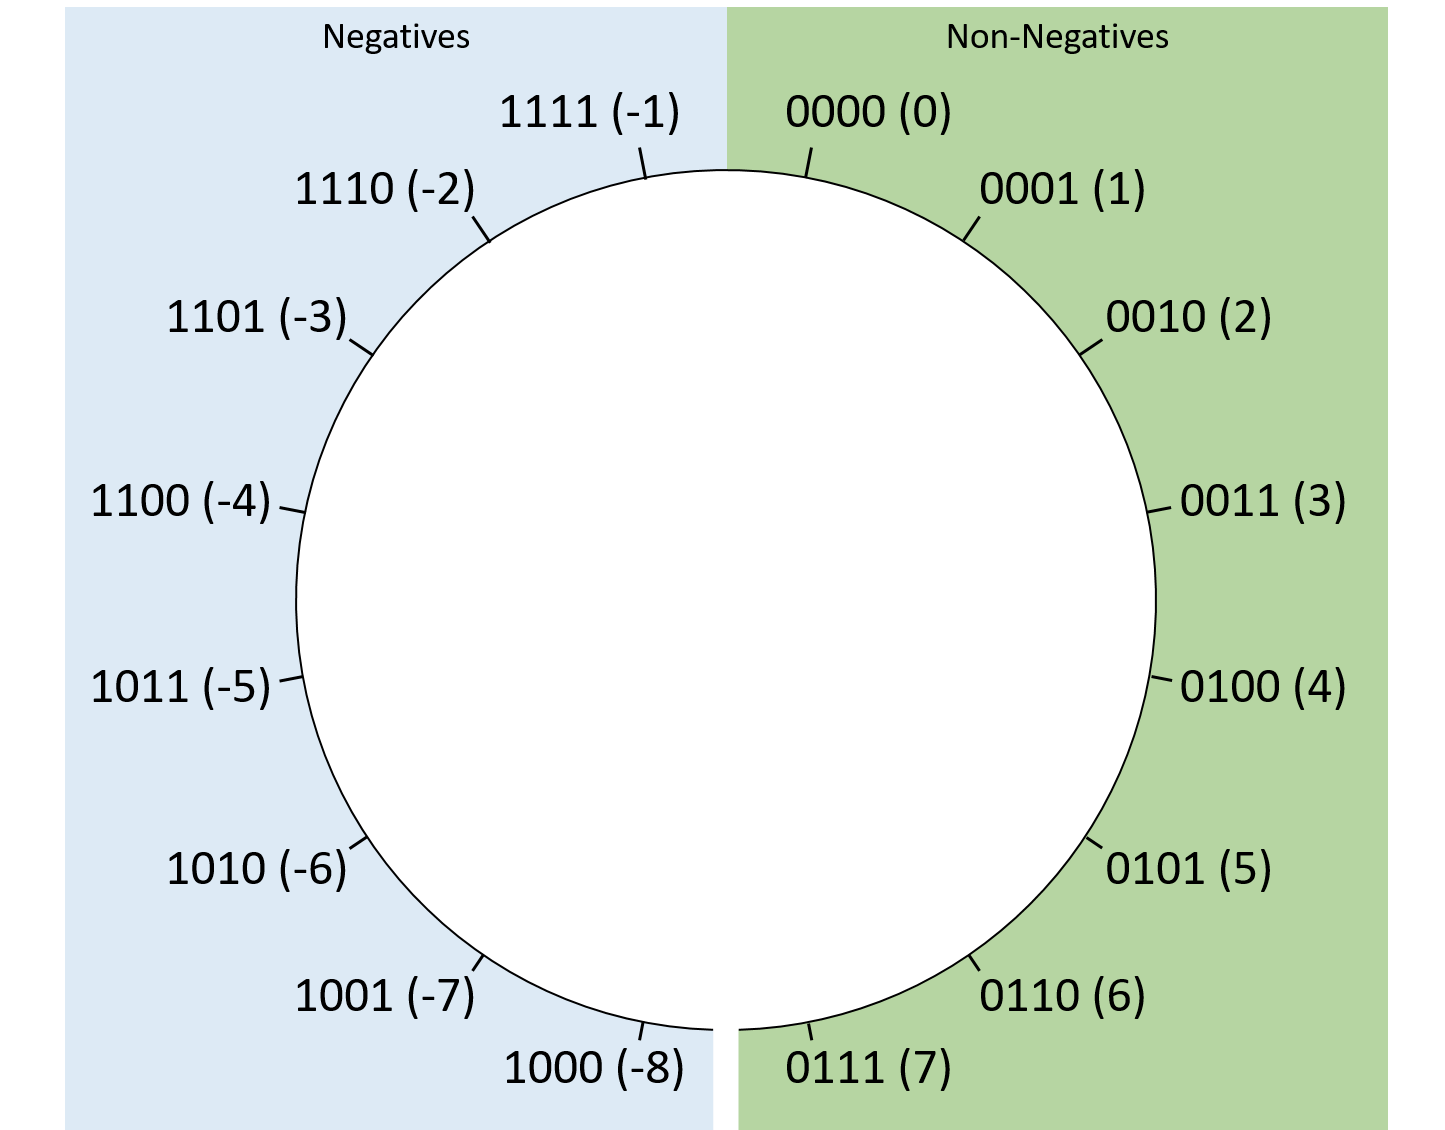
\includegraphics[width=0.41\textwidth]{circle-twoscomplement.png} % Replace 'path_to_image.png' with the actual path to your image file
  \caption{Circular representation of two's complement}
\end{wrapfigure}

In two's complement arithmetic, a circular graphical representation can be used to illustrate the addition and subtraction of numbers:
\begin{itemize}
  \item[-] Moving \textbf{clockwise} from 0 represents the \textit{addition} of positive numbers.
  \item[-] Moving \textbf{counterclockwise} represents the \textit{subtraction} of positive numbers.
  \item[-] Crossing the line where the sign changes indicates a \textit{change of sign} from positive to negative or vice versa.
  \item[] \textbf{Examples:}
    \begin{itemize}
        \item[] The addition of two positive numbers, such as \(2 + 3\), is shown by moving clockwise from 0 to 2 and then moving 3 more steps clockwise, resulting in 5.
        \item[] The subtraction of a smaller number from a larger number, such as \(5 - 3\), is shown by moving clockwise from 0 to 5 and then moving 3 steps counterclockwise, resulting in 2.  
    \end{itemize}
\end{itemize}

\subsection{Addition and Subtraction}
\subsection{Addition}
Given two \(n\)-bit numbers \(A\) and \(B\), their sum in two's complement arithmetic is obtained by directly adding them together as binary numbers:
\begin{equation}
    \text{Sum} = A + B
\end{equation}
If there is an overflow, i.e., a carry out of the most significant bit (MSB), it is discarded. The result is also represented in \(n\) bits.

\subsection{Subtraction}
To subtract one \(n\)-bit number \(B\) from another \(A\) using two's complement arithmetic, convert \(B\) to its two's complement and then add it to \(A\):
\begin{enumerate}
    \item Find the two's complement of \(B\), denoted as \(\bar{B}\), by inverting all the bits of \(B\) and adding \(1\).
    \item Add \(A\) to the two's complement of \(B\):
    \begin{equation}
        \text{Difference} = A + \bar{B}
    \end{equation}
\end{enumerate}
As with addition, discard any overflow from the MSB.


\section{Binary Multiplication}

\begin{proof}[Proof]
    Let $X$ and $Y$ be two numbers, then their product can be represented as:
    \begin{align*}
    X \cdot Y &= X \cdot \left( -Y_{n-1} \cdot 2^{n-1} + X \sum_{i=0}^{n-2} Y_i \cdot 2^i \right) \\
    &= -X \cdot Y_{n-1} \cdot 2^{n-1} + X \sum_{i=0}^{n-2} Y_i \cdot 2^i \\
    &= -Y_{n-1} \cdot X \cdot 2^{n-1} + Y_{n-2} \cdot X \cdot 2^{n-2} + \ldots + Y_2 \cdot X \cdot 2^2 + Y_1 \cdot X \cdot 2^1 + Y_0 \cdot X \cdot 2^0
    \end{align*}
\end{proof}
    
  

\newpage
Binary multiplication operates similarly to decimal multiplication but is performed bit by bit. Here is a clearer example illustrating the multiplication of two binary numbers:

\begin{align*}
    & \text{Multiplicand} & 1101 & \quad & \text{(This is the number to be multiplied)}\\
    & \text{Multiplier} & \times \; 0011 & & \text{(This number multiplies the multiplicand)}\\
    \cline{2-4}
    && 1101 & & \text{(Multiply by 1, the least significant bit of the multiplier)}\\
    &+& 11010 & & \text{(Multiply by 1, add one zero to the right, (left shift, $<<1$))}\\
    &+& 000000 & & \text{(Multiply by 0, add two zeros to the right, (left shift, $<<2$))}\\
    &+& 0000000 & & \text{(Multiply by 0, add three zeros to the right, (left shift, $<<3$))}\\
    \cline{2-4}
    && 1000111 & & \text{(Sum of the partial products)}
\end{align*}




\chapter{Number Systems (Part III)}
Incoming...

\end{document}
